% Native editable composition from verified, unchanged IDE images.
\par
\begin{figure}[htbp]
  \centering
  \sbox0{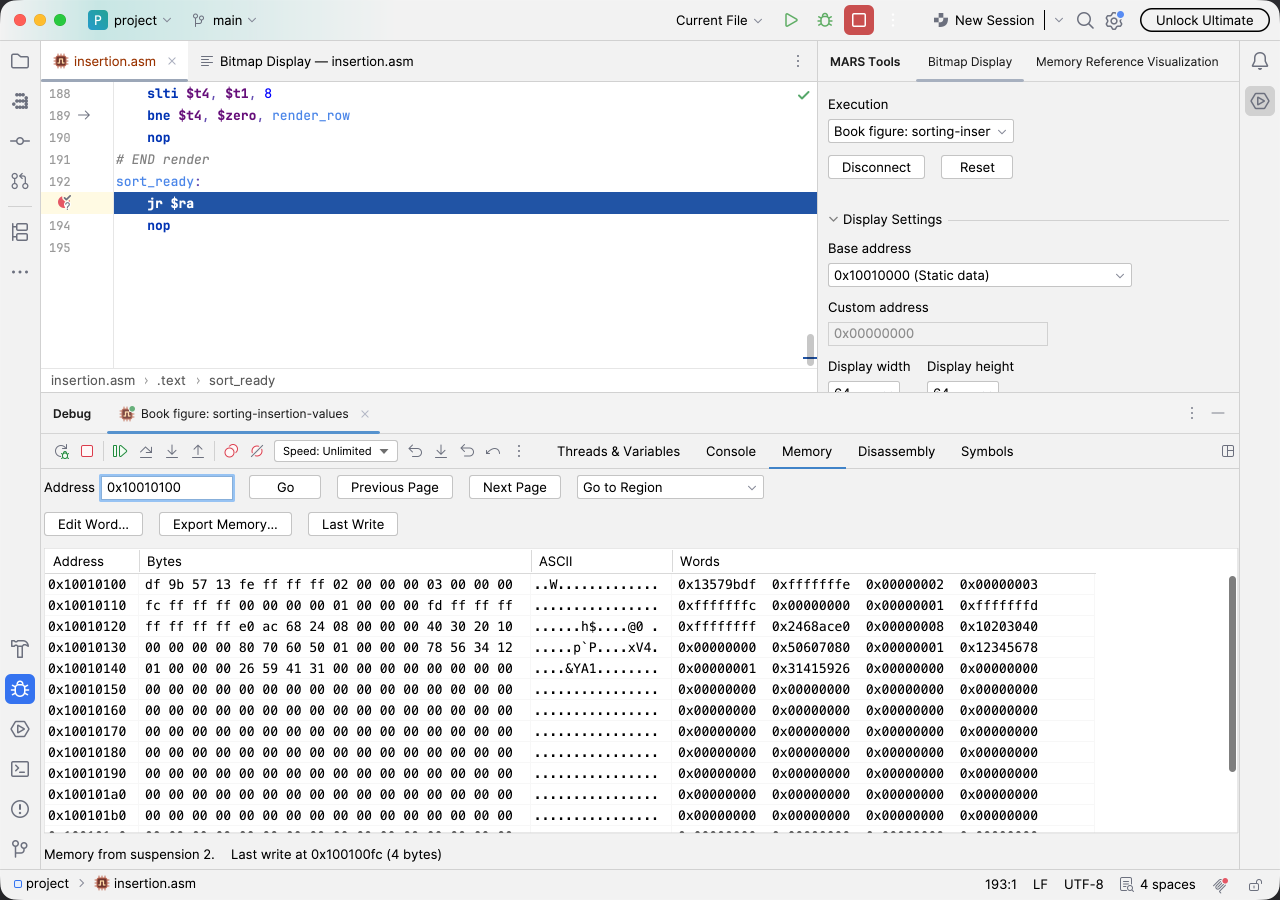
\includegraphics[artifact]{packages/009-sorting-visualizer/captures/f02-insertion/values.png}}
  \sbox2{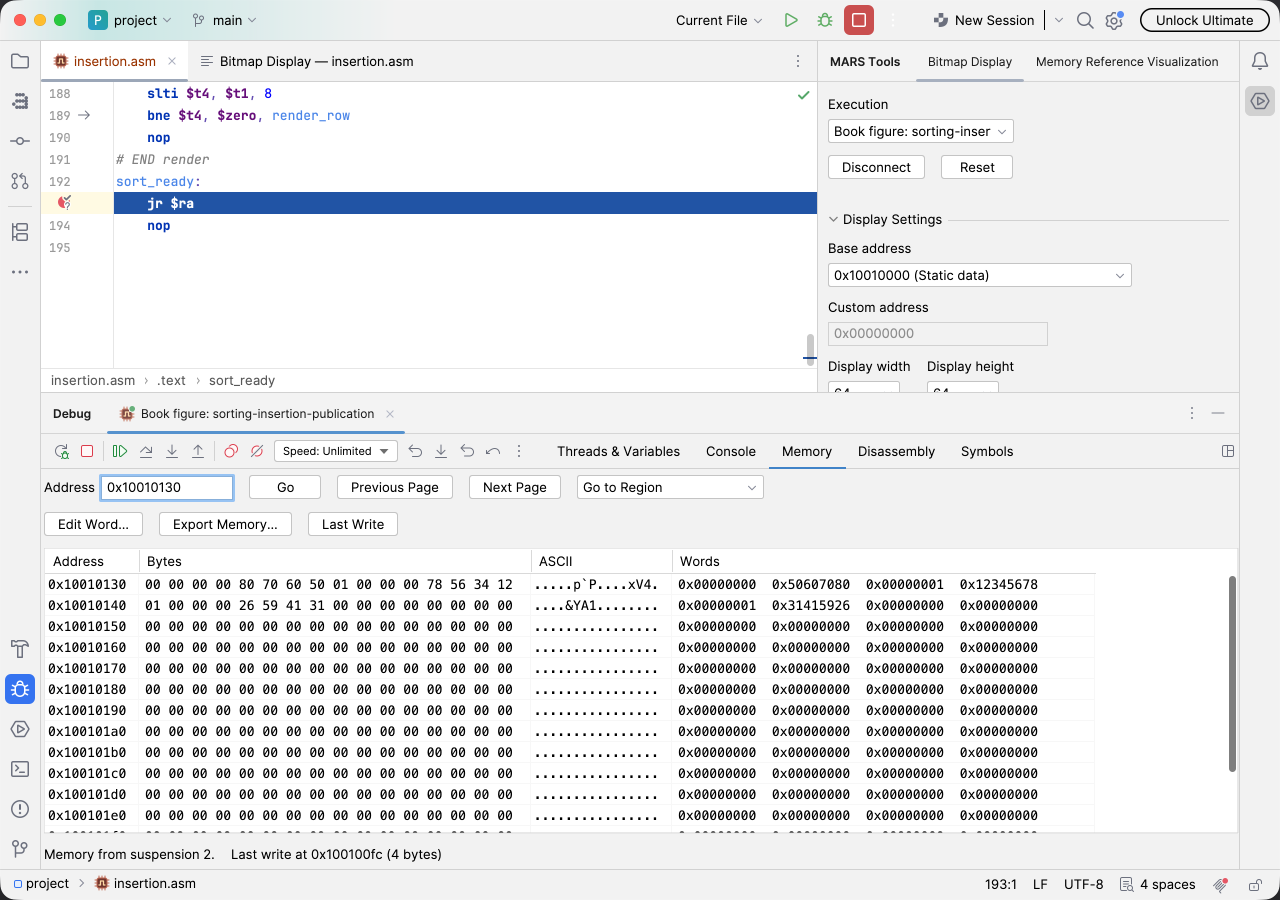
\includegraphics[artifact]{packages/009-sorting-visualizer/captures/f02-insertion/publication.png}}
  \sbox4{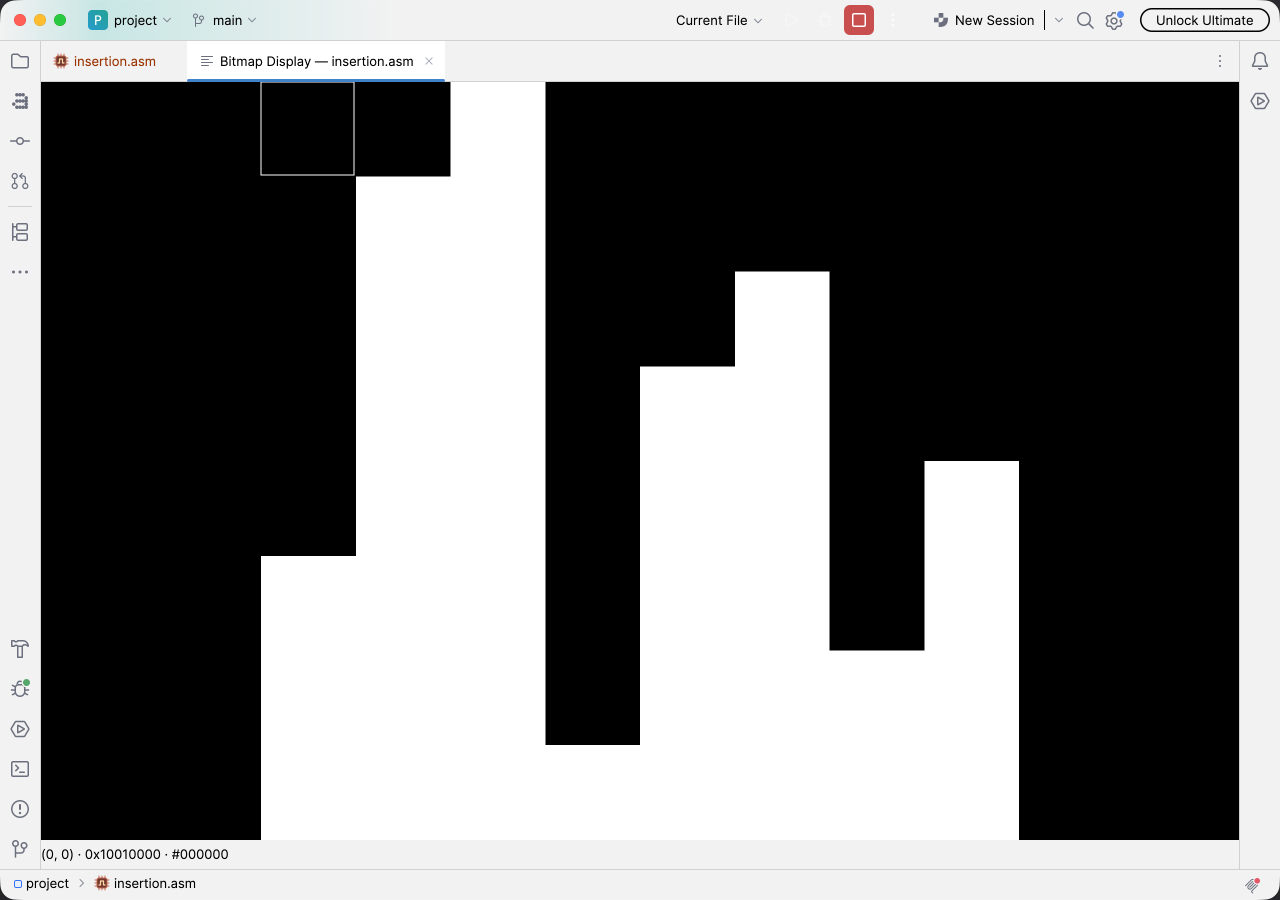
\includegraphics[artifact]{packages/009-sorting-visualizer/captures/f02-insertion/bitmap.png}}
  \edef\MARSinsertionsourceLeft{\the\dimexpr0.036718750\wd0\relax}
  \edef\MARSinsertionsourceBottom{\the\dimexpr0.757777778\ht0\relax}
  \edef\MARSinsertionsourceRight{\the\dimexpr0.611718750\wd0\relax}
  \edef\MARSinsertionsourceTop{\the\dimexpr0.164444444\ht0\relax}
  \edef\MARSinsertionstateLeft{\the\dimexpr0.034375000\wd0\relax}
  \edef\MARSinsertionstateBottom{\the\dimexpr0.287777778\ht0\relax}
  \edef\MARSinsertionstateRight{\the\dimexpr0.578906250\wd0\relax}
  \edef\MARSinsertionstateTop{\the\dimexpr0.608888889\ht0\relax}
  \edef\MARSinsertionmemoryLeft{\the\dimexpr0.034375000\wd2\relax}
  \edef\MARSinsertionmemoryBottom{\the\dimexpr0.311111111\ht2\relax}
  \edef\MARSinsertionmemoryRight{\the\dimexpr0.578906250\wd2\relax}
  \edef\MARSinsertionmemoryTop{\the\dimexpr0.608888889\ht2\relax}
  \edef\MARSinsertionplotLeft{\the\dimexpr0.203906250\wd4\relax}
  \edef\MARSinsertionplotBottom{\the\dimexpr0.066666667\ht4\relax}
  \edef\MARSinsertionplotRight{\the\dimexpr0.203906250\wd4\relax}
  \edef\MARSinsertionplotTop{\the\dimexpr0.091111111\ht4\relax}
  \begin{tikzpicture}[alt={Four annotated details after the first adjacent insertion exchange. The signed array is minus two, two, three, minus four, zero, one, minus three, minus one. Selector zero chooses insertion. Phase and exchange count are one. Only columns zero and one change from the original frame, to heights three and seven.}]
    \node[anchor=north west,inner sep=0,font=\small\bfseries] (source-title) at (6mm,0) {Next instruction: return from the renderer};
    \node[anchor=north west,inner sep=0] (source) at ([yshift=-1mm]source-title.south west) {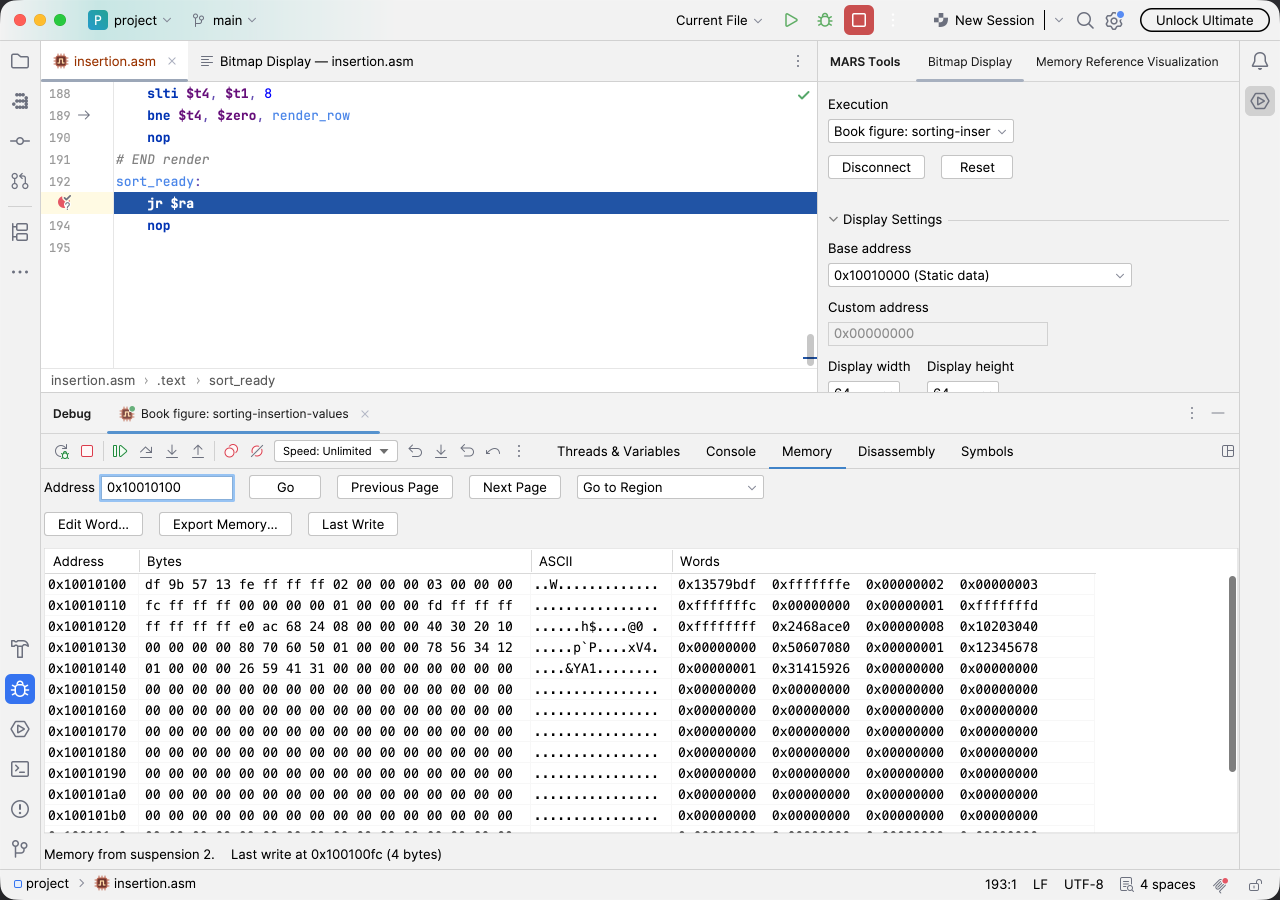
\includegraphics[width=0.7\linewidth,artifact,trim={\MARSinsertionsourceLeft{} \MARSinsertionsourceBottom{} \MARSinsertionsourceRight{} \MARSinsertionsourceTop{}},clip]{packages/009-sorting-visualizer/captures/f02-insertion/values.png}};
    \begin{scope}[shift={(source.south west)},x={($(source.south east)-(source.south west)$)},y={($(source.north west)-(source.south west)$)}]
      \draw[black,line width=0.7pt] (0.153333333,0.057142857) rectangle (0.326666667,0.371428571);
      \node[draw=black,fill=white,circle,inner sep=1.5pt,font=\footnotesize] at ($(0.153333333,0.371428571)+(-3mm,0)$) {1};
    \end{scope}
    \node[anchor=north west,inner sep=0,font=\small\bfseries] (state-title) at ([yshift=-1mm]source.south west) {Signed array words and neighboring guards};
    \node[anchor=north west,inner sep=0] (state) at ([yshift=-1mm]state-title.south west) {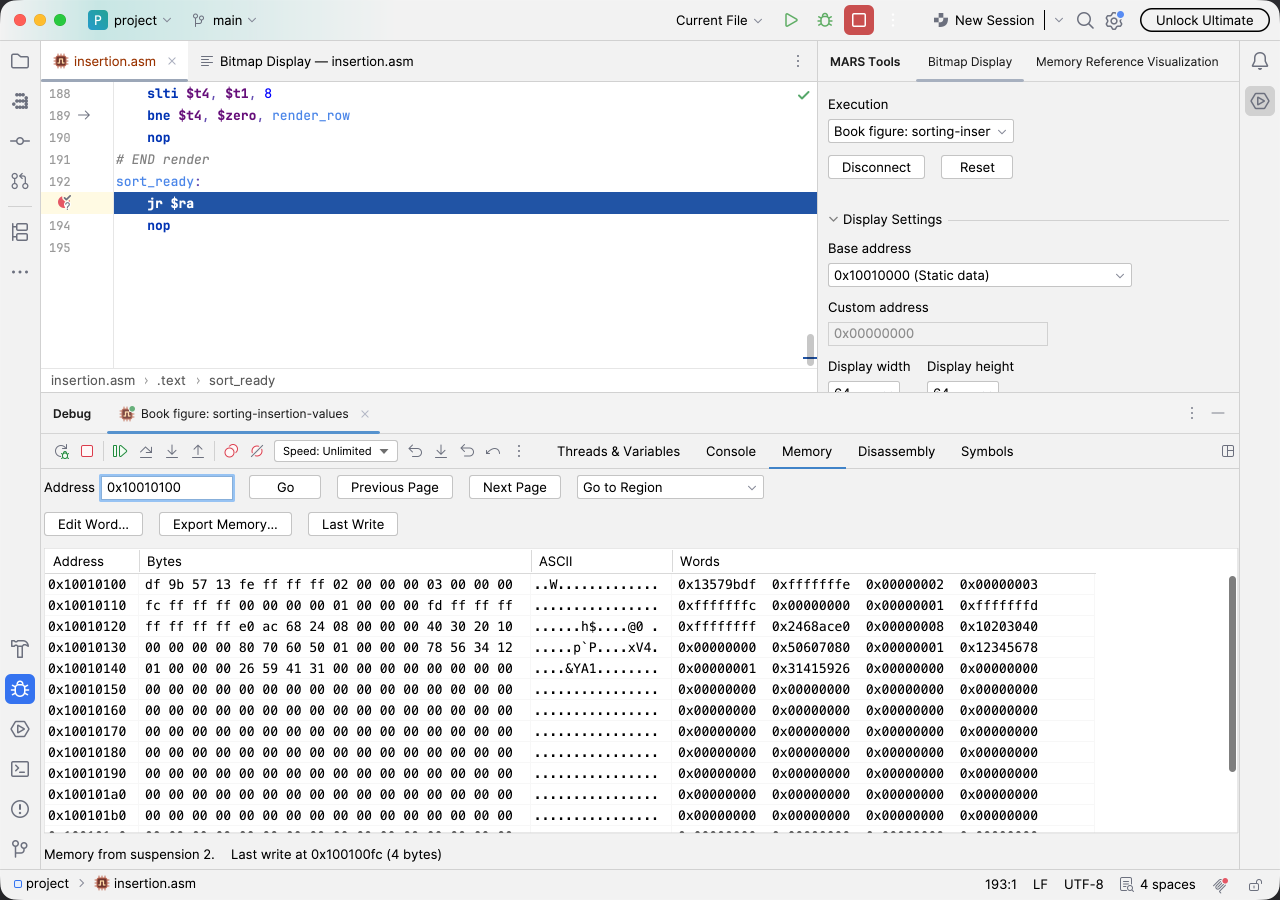
\includegraphics[width=0.78\linewidth,artifact,trim={\MARSinsertionstateLeft{} \MARSinsertionstateBottom{} \MARSinsertionstateRight{} \MARSinsertionstateTop{}},clip]{packages/009-sorting-visualizer/captures/f02-insertion/values.png}};
    \begin{scope}[shift={(state.south west)},x={($(state.south east)-(state.south west)$)},y={($(state.north west)-(state.south west)$)}]
      \draw[black,line width=0.7pt] (0.191919192,0.043010753) rectangle (0.983838384,0.720430108);
      \node[draw=black,fill=white,circle,inner sep=1.5pt,font=\footnotesize] at ($(0.191919192,0.720430108)+(-3mm,0)$) {2};
    \end{scope}
    \node[anchor=north west,inner sep=0,font=\small\bfseries] (memory-title) at ([yshift=-1mm]state.south west) {Algorithm, phase and completed-exchange count};
    \node[anchor=north west,inner sep=0] (memory) at ([yshift=-1mm]memory-title.south west) {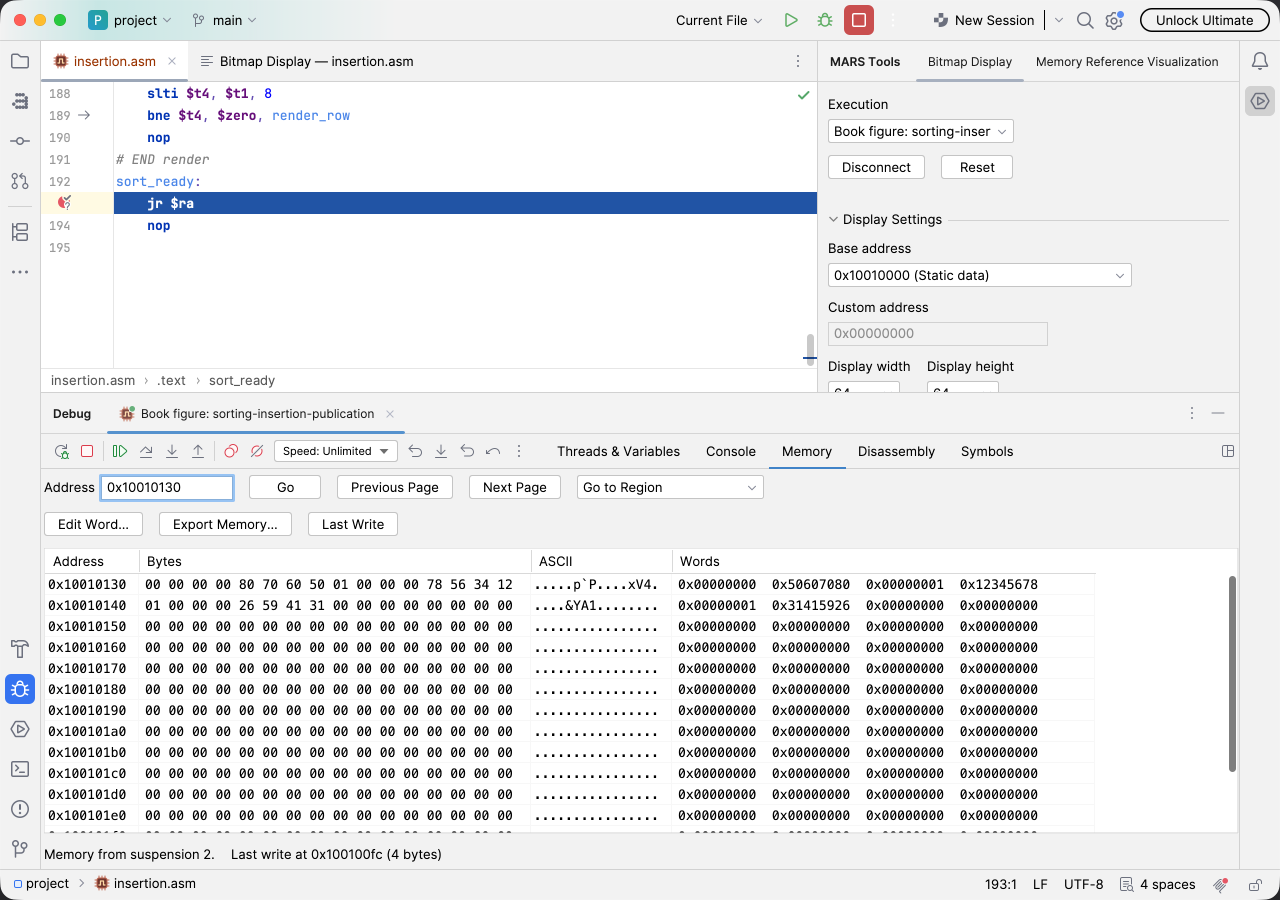
\includegraphics[width=0.78\linewidth,artifact,trim={\MARSinsertionmemoryLeft{} \MARSinsertionmemoryBottom{} \MARSinsertionmemoryRight{} \MARSinsertionmemoryTop{}},clip]{packages/009-sorting-visualizer/captures/f02-insertion/publication.png}};
    \begin{scope}[shift={(memory.south west)},x={($(memory.south east)-(memory.south west)$)},y={($(memory.north west)-(memory.south west)$)}]
      \draw[black,line width=0.7pt] (0.191919192,0.055555556) rectangle (0.983838384,0.638888889);
      \node[draw=black,fill=white,circle,inner sep=1.5pt,font=\footnotesize] at ($(0.191919192,0.638888889)+(-3mm,0)$) {3};
    \end{scope}
    \node[anchor=north west,inner sep=0,font=\small\bfseries] (plot-title) at ([yshift=-1mm]memory.south west) {Complete published framebuffer};
    \node[anchor=north west,inner sep=0] (plot) at ([yshift=-1mm]plot-title.south west) {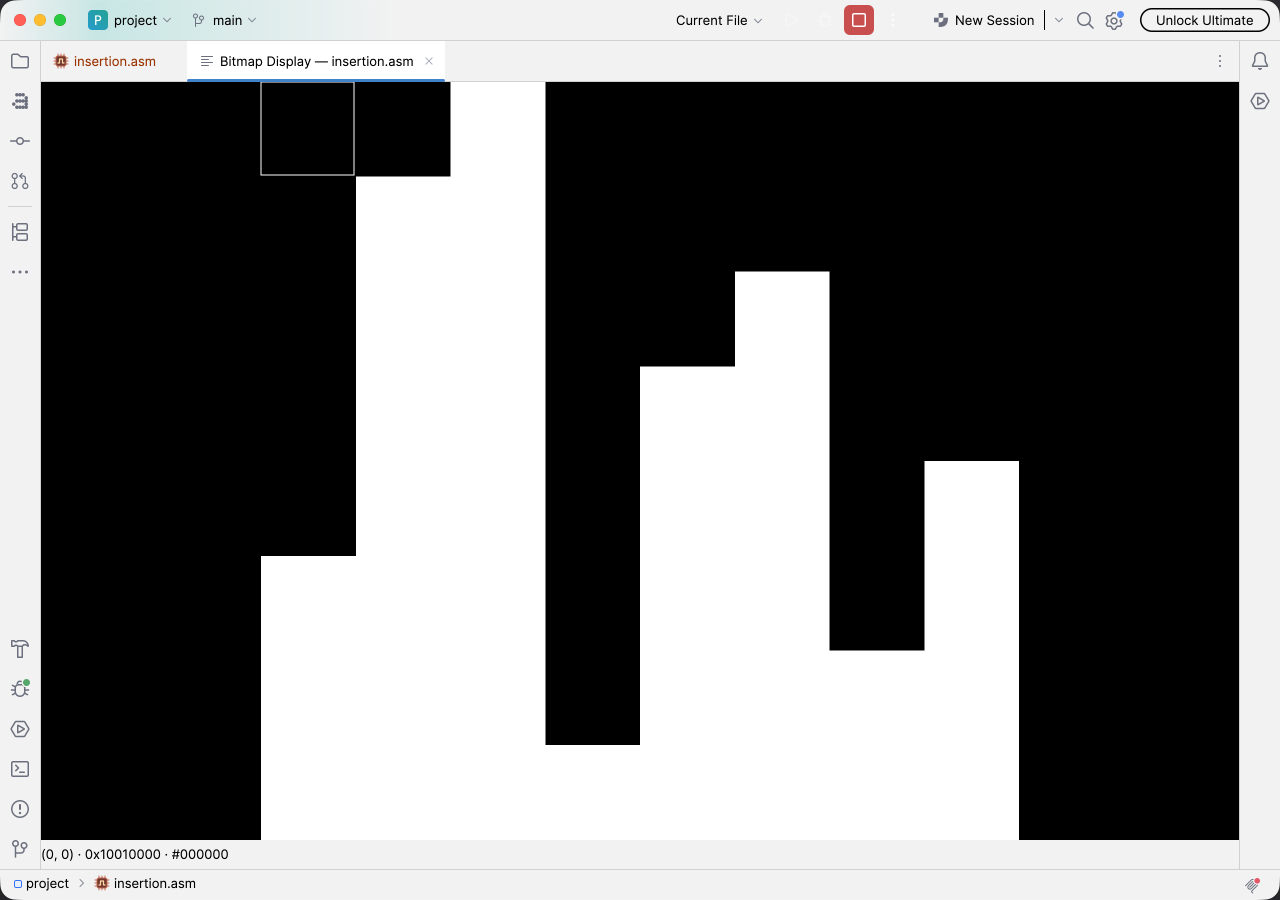
\includegraphics[width=0.24\linewidth,artifact,trim={\MARSinsertionplotLeft{} \MARSinsertionplotBottom{} \MARSinsertionplotRight{} \MARSinsertionplotTop{}},clip]{packages/009-sorting-visualizer/captures/f02-insertion/bitmap.png}};
    \begin{scope}[shift={(plot.south west)},x={($(plot.south east)-(plot.south west)$)},y={($(plot.north west)-(plot.south west)$)}]
      \draw[black,line width=0.7pt] (0.000000000,0.000000000) rectangle (1.000000000,1.000000000);
      \node[draw=black,fill=white,circle,inner sep=1.5pt,font=\footnotesize] at ($(0.000000000,1.000000000)+(-3mm,0)$) {4};
      \foreach \c in {0,...,7} {\node[anchor=north,font=\scriptsize,inner sep=0] at ({(\c+0.5)/8},-0.035) {\c}; \node[anchor=east,font=\scriptsize,inner sep=0] at (-0.025,{1-(\c+0.5)/8}) {\c};}
      \node[anchor=north,font=\scriptsize,inner sep=0] at (0.5,-0.11) {$x$}; \node[anchor=east,font=\scriptsize,inner sep=0] at (-0.10,0.5) {$y$};
    \end{scope}
  \end{tikzpicture}
  \par\smallskip
  \begin{minipage}{\linewidth}
    \small
    \begin{enumerate}
      \item The condition \texttt{\$s6 == 1} selects the first completed-exchange frame at \texttt{sort\_ready}. The renderer is paused before returning to the insertion loop; no second exchange has begun.
      \item The array is now $[-2,2,3,-4,0,1,-3,-1]$. The first two words exchanged places: \texttt{fe ff ff ff} is followed by \texttt{02 00 00 00}. Both loads and both stores completed before the count update and renderer call. The remaining six values retain their original order.
      \item Selector 0 still names insertion sort. Phase 1 and exchange count 1 describe this complete exchange. At the earlier \texttt{insertion\_swapped} boundary, the array already had these words, while the count was still 0 and the framebuffer still showed the original order. Redrawing brought the image into agreement.
      \item Column 0 shrinks from seven white cells to three; column 1 grows from three to seven. Their new first white rows are 5 and 1. The other six columns are unchanged. The renderer writes black words as well as white ones, so the old upper portion of column 0 is cleared.
    \end{enumerate}
  \end{minipage}
  \caption{The first insertion exchange is complete and its new frame is published.}
  \label{capture:009-sorting-visualizer-f02-insertion}
\end{figure}
\par
